\textbf{COLUNI 2024 -- Questão 02}\par\medskip Leia os textos abaixo para responder às questões 1, 2 e 3.

\textbf{Texto I}

\begin{center}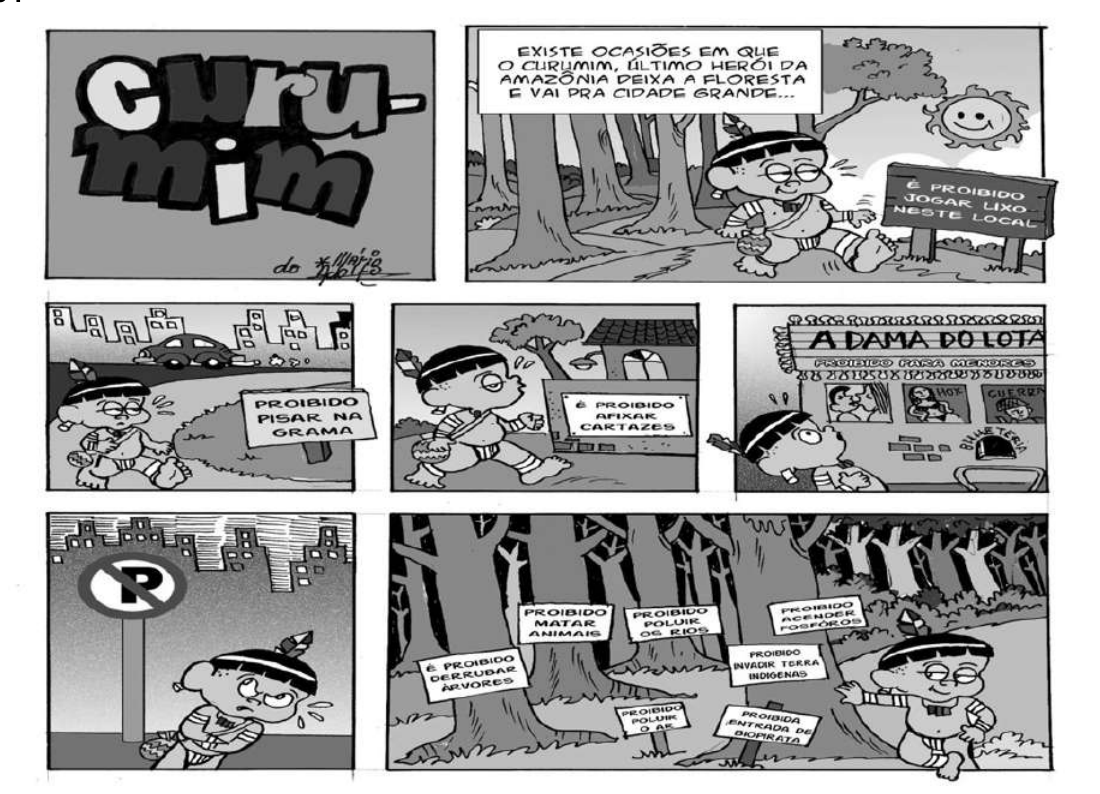
\includegraphics[width=0.90\linewidth]{static/simulados/coluni/figuras/2024/questao-02/figura-1.png}\end{center}
Disponível em: https://marioadolfo.com/festa-na-floresta-curumim-o-ultimo-heroi-da-amazonia-completa-37-anos/. Acesso em: 05 set. 2023.

\textbf{Texto II}

\begin{center}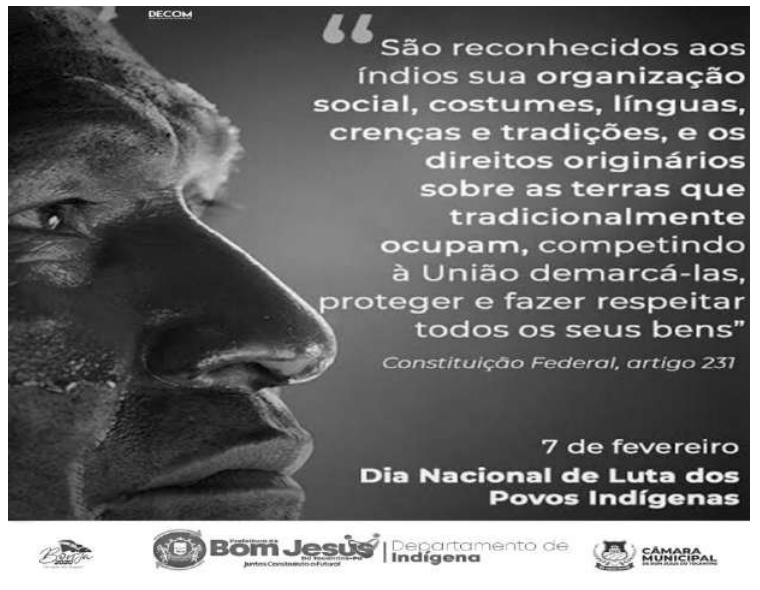
\includegraphics[width=0.68\linewidth]{static/simulados/coluni/figuras/2024/questao-02/figura-2.png}\end{center}
Disponível em: https://bomjesusdotocantins.pa.gov.br/dia-nacional-de-luta-dos-povos-indigenas/. Acesso em: 19 set. 2023.

De acordo com a leitura e análise dos textos I e II, é CORRETO o que se afirma em:
\begin{enumerate}
\item No texto I, as orientações da cidade grande estão materializadas em linguagem verbal e não verbal,
       enquanto, no texto II, há um artigo da constituição retextualizado em linguagem verbal.
\item No texto I, as orientações da cidade grande estão materializadas, exclusivamente, na forma verbal, no
       texto II é possível reconhecer, na parte não verbal, uma representação indígena para compor o post.
\item No texto I, as orientações da cidade grande estão situadas em espaços coletivos, já no texto II, a autoria
       do anúncio publicitário é individual, e refere-se à prefeitura de Bom Jesus do Tocantins.
\item No texto I, as orientações da cidade grande foram transferidas na íntegra para a floresta, no texto II, a
       orientação do artigo constitucional foi modificada para ilustrar o discurso institucional da prefeitura.
\end{enumerate}
